\documentclass[conference]{IEEEtran}
\usepackage{cite}
\usepackage{amsmath,amssymb,amsfonts}
\usepackage{algorithmic}
\usepackage{graphicx}
\usepackage{textcomp}
\usepackage{xcolor}
\usepackage{booktabs}
\usepackage{float}
\usepackage{hyperref}


\def\BibTeX{{\rm B\kern-.05em{\sc i\kern-.022em b}\kern-.08em
    T\kern-.1667em\lower.7ex\hbox{E}\kern-.125emX}}

\begin{document}

\title{Visualization Tool for Energy Analysts using CIA Dataset}
\author{
    Harshavardhan Dharman\\
    \scriptsize Eindhoven University of Technology\\
    \scriptsize h.dharman@student.tue.nl
\and
    Surya Kannan\\
    \scriptsize Eindhoven University of Technology\\
    \scriptsize s.kannan@student.tue.nl
\and
    Shashank Venkatesha\\
    \scriptsize Eindhoven University of Technology\\
    \scriptsize s.venkatesha@student.tue.nl
\and
    Leela Karthikeyan Haribabu\\
    \scriptsize Eindhoven University of Technology\\
    \scriptsize l.k.haribabu@student.tue.nl
}



\maketitle
{\color{blue}
\begin{abstract}
We built an interactive visualization tool for energy analysts to explore the CIA World Factbook dataset. Our tool combines data from five domains energy, economy, demographics, transport, and geography covering over 200 countries. Users can view global patterns on a choropleth map, compare countries using scatter plots and bar charts, and find similar nations through PCA clustering. All views are linked: clicking a country on the map highlights it in all other charts, and brushing in parallel coordinates filters the data across views. We found that $CO_2$ emissions are heavily concentrated in five countries, and discovered a 0.46 correlation between GDP and electricity access showing that wealth alone does not ensure infrastructure. The tool supports Shneiderman's mantra of overview first, then zoom and filter, then details-on-demand. This enables analysts to explore relationships and form their own insights interactively.
\end{abstract}
}

\begin{IEEEkeywords}
Energy Analytics, Information Visualization, Multivariate Profiling, Infrastructure Assessment, PCA Clustering.
\end{IEEEkeywords}
{\color{blue}
\section{Introduction}
\subsection{Motivation and Domain Problem}
Energy analysts need to understand how energy production connects to economic development across countries. The CIA World Factbook provides data on over 200 countries covering energy, economy, demographics, transport, and geography. However, analyzing this data in spreadsheets is difficult because patterns like ``high GDP with high carbon emissions'' or ``electricity access gaps despite economic growth'' are hidden in rows of numbers. Our goal is to build a tool for exploration and analysis that lets analysts discover these patterns visually. This problem is relevant because energy infrastructure decisions affect billions of people. Understanding which countries succeed or fail at providing electricity despite similar resources can inform policy. Thus, this visualization tool combines all five domains (energy, economy, demographics, transport, geography) in one linked interface for this type of cross-sectoral analysis.

\subsection{Target Users and Goals}
\textbf{Target User:} Energy analysts who synthesize multi-sector data for infrastructure planning and policy decisions.

\textbf{Goal:} Enable exploration of global energy data to: \\(1) compare countries by energy and economic indicators, \\(2) identify groups of similar countries using clustering, and \\(3) find outliers countries that perform unusually well or poorly given their resources.

\subsection{Why Visualization?}
Visualization is better than statistical methods alone because the human eye can recognize patterns that algorithms miss. A choropleth map immediately shows which regions lack electricity. A scatter plot reveals whether GDP correlates with energy access. Statistics can summarize data, but visualization lets analysts form and test their own hypotheses. Our tool follows Shneiderman's mantra: overview first, then zoom and filter, then details-on-demand.
}
\section{Data Analysis}

\subsection{Domain Data Specification}
The visualization uses the CIA World Factbook, which contains data on over 200 countries across five domains. Nations are analyzed through these dimensions:

\textbf{Energy:} Tracks energy usage through electricity access, generating capacity, and fossil fuel metrics (coal, gas, petroleum). $CO_2$ emissions show industrial output.

\textbf{Economy:} Shows economic indicators using Real GDP (PPP) and Trade Volume (Exports/Imports), plus GDP per Capita for relative wealth.

\textbf{Demographics:} Uses Total Population to understand energy demand and infrastructure scale needed.

\textbf{Transportation:} Covers gas and oil pipeline mileage (km), showing how developed a nation's distribution networks are.

\textbf{Geography:} Includes Total/Land Area and land-use types like Forest and Agricultural Land to understand spatial context.

We merged five datasets (Energy, Economy, Demographics, Transportation, Geography) into one table. Each row represents a country, identified by its ISO-Alpha 3 code. We matched country names between the CIA World Factbook and Gapminder ISO database to resolve naming differences (e.g., ``Czechia'' to ``Czech Republic'').

\textcolor{blue}{\textbf{Missing Values:} Approximately 15\% of country-indicator pairs contain missing values. We exclude countries with missing data from specific visualizations rather than imputing, to preserve accuracy.}

\textcolor{blue}{\textbf{Derived Attributes:} We created two derived attributes: (1) \texttt{iso\_alpha} for geographic mapping and cross-dataset joining, and (2) \texttt{continent} for regional filtering, inferred using the pycountry-convert library.}

\subsection{Data Abstraction}
Following Munzner's framework, we classify each attribute by semantic type (what it represents) and data type (how it can be compared). The tables below show our abstraction:

\begin{table}[H]
\centering
\caption{Energy Dataset Abstraction}
\label{tab:data_abstraction}
\small
\begin{tabular}{|p{3.7cm}|p{1.5cm}|p{0.9cm}|p{1.4cm}|}
\hline
\textbf{Attribute} & \textbf{Semantic Type} & \textbf{Data Type} & \textbf{Range} \\
\hline
Country & Categorical & Key (Item) & 260 unique \\
electricity\_access\_percent & Quantitative & Ratio & 0--100\% \\
elec\_generating\_capacity\_kW & Quantitative & Ratio & 0--2.38B \\
coal\_metric\_tons & Quantitative & Ratio & 0--3.69B \\
petroleum\_bbl\_per\_day & Quantitative & Ratio & 0--18.6M \\
refined\_petrol\_products & Quantitative & Ratio & 0--20.3M \\
refined\_petrol\_exports & Quantitative & Ratio & 0--5.92M \\
refined\_petrol\_imports & Quantitative & Ratio & 0--2.19M \\
natural\_gas\_cubic\_m & Quantitative & Ratio & 0--967B \\
carbon\_dioxide\_emissions & Quantitative & Ratio & 0--11.5B Mt \\
iso\_alpha (derived) & Categorical & Key & 200+ unique \\
continent (derived) & Categorical & Ordered & 6 categories \\
\hline
\end{tabular}
\end{table}

\begin{table}[H]
\centering
\caption{Economy Dataset Abstraction}
\small
\begin{tabular}{|l|l|l|l|}
\hline
\textbf{Attribute} & \textbf{Semantic Type} & \textbf{Data Type} & \textbf{Range} \\
\hline
Real GDP (PPP) & Quantitative & Ratio & 0--23,320 \\
GDP per Capita & Quantitative & Ratio & 0--115,700 \\
Exports (B USD) & Quantitative & Ratio & 0--3,527 \\
Imports (B USD) & Quantitative & Ratio & 0--3,401 \\
\hline
\end{tabular}
\end{table}

\begin{table}[H]
\centering
\caption{Demographics Dataset Abstraction}
\small
\begin{tabular}{|l|l|l|l|}
\hline
\textbf{Attribute} & \textbf{Semantic Type} & \textbf{Data Type} & \textbf{Range} \\
\hline
Total Population & Quantitative & Absolute & 0--1.42B \\
\hline
\end{tabular}
\end{table}

\begin{table}[h]
\centering
\caption{Geography Dataset Abstraction}
\small
\begin{tabular}{|l|l|l|p{1.1cm}|}
\hline
\textbf{Attribute} & \textbf{Semantic Type} & \textbf{Data Type} & \textbf{Range} \\ \hline
Area\_Total & Quantitative & Ratio & 0-17.1M sq km \\
Land\_Area & Quantitative & Ratio & 0-16.3M sq km \\
Forest\_Land & Quantitative & Ratio & 0-100\% \\
Agricultural\_Land & Quantitative & Ratio & 0-100\% \\ \hline
\end{tabular}
\end{table}


\section{Task Analysis}

\subsection{Task Hierarchy}
{\color{blue}
Following Munzner's recommendation, we organize tasks from high-level goals to low-level actions. This hierarchy ensures our visualization supports both strategic analysis and detailed data retrieval.

\textbf{High-Level Goal:} Understand how energy production connects to economic development across countries. This requires synthesizing patterns across multiple indicators and regions.

\textbf{Mid-Level Tasks:}
\begin{enumerate}
    \item Analyze emissions patterns to identify major polluters
    \item Correlate economic wealth with energy access
    \item Identify countries with high carbon intensity relative to GDP
    \item Discover regional clusters with similar energy profiles
\end{enumerate}

\textbf{Low-Level Tasks:}
\begin{itemize}
    \item \textbf{Lookup}: Retrieve exact values for a specific country (hover tooltip shows precise numbers)
    \item \textbf{Filter}: Reduce visible data by region or attribute range
    \item \textbf{Select}: Pick individual countries for detailed comparison
    \item \textbf{Compare}: Evaluate two or more countries side-by-side on specific metrics 
    \item \textbf{Browse}: Scan through multivariate profiles to spot patterns 
    \item \textbf{Locate}: Find a country's position on the map 
\end{itemize}
}
\subsection{Task Abstraction}

Following Munzner’s task abstraction framework, we reformulate domain-specific analytical goals into abstract action--target pairs. This process removes domain terminology (e.g., ``GDP'' or ``carbon emissions'') and replaces it with generic analytical objectives such as identifying extremes, exploring distributions, and analyzing relationships. Task abstraction allows us to systematically match user goals with appropriate visualization and interaction techniques during visualization.

\paragraph{Identify Extremes (Action: Identify \;|\; Target: Extremes)}
To identify extreme values within the data by investigating through trends and patterns in data. This supports the task of identifying items that exhibit unusually high values relative to others. The visualization enables quick recognition of entities that deviate strongly from the overall distribution, highlighting outliers that warrant further investigation.

\paragraph{Locate and Discover Spatial Distribution (Action: Locate \;|\; Target: Spatial Distribution)}
To examine how values are distributed across geographic space. Spatial data is used to analyze the distribution of quantitative attributes and discover regional patterns. By observing areas with relatively high or low values, the analyst can identify spatial clusters and disparities that are not apparent from non-spatial views.

\paragraph{Analyze Dependencies (Action: Analyze \;|\; Target: Correlation)}
Investigate relationships among multiple quantitative attributes to analyze correlations and dependencies, including identifying whether relationships are strong, weak, or non-linear. Compare these relationships across different subsets of the data to reveal patterns, trends, or anomalies, and to understand how attributes influence each other within different regions or groups.

\subsection{Domain-Specific Tasks}
\textbf{Task 1: Analyze Environmental Impact and Global Emissions}
\begin{itemize}
    \item \textbf{Description}: Identifying drivers of greenhouse gas emissions by analyzing $CO_{2}$ output in relation to industrial scale (see Fig.~\ref{fig:global_emissions}).
    \item \textbf{Questions}: Who are the leading global carbon emitters? Which countries contribute most to global $CO_{2}$ emissions? Is there a correlation between electricity capacity and carbon output?
    \item \textbf{Insights}: China and the United States of America have extensive access to electricity globally. As a result, these two countries have high $CO_{2}$ emissions because they consume a significantly large amount of electricity
\end{itemize}

% Using [H] to lock the figure precisely after the list
\begin{figure}[H]
    \centering
    % Note: It is best practice to avoid spaces in filenames, e.g., fig_2.jpeg
    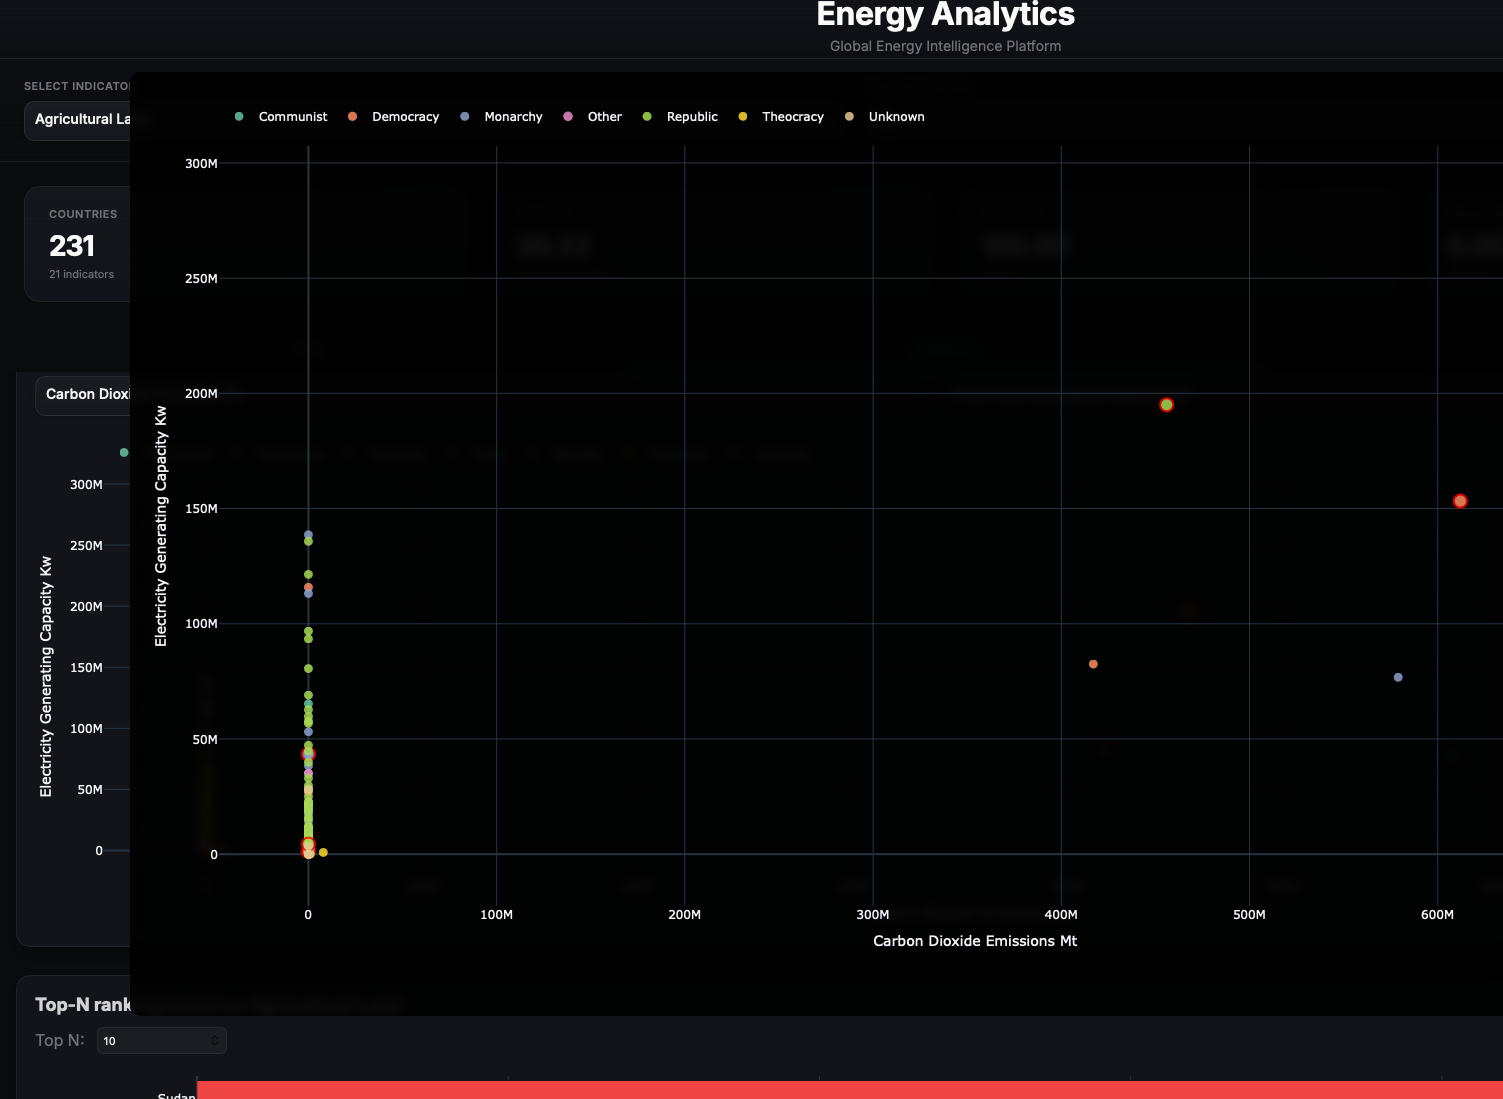
\includegraphics[width=1.0\linewidth]{img15.png}
    %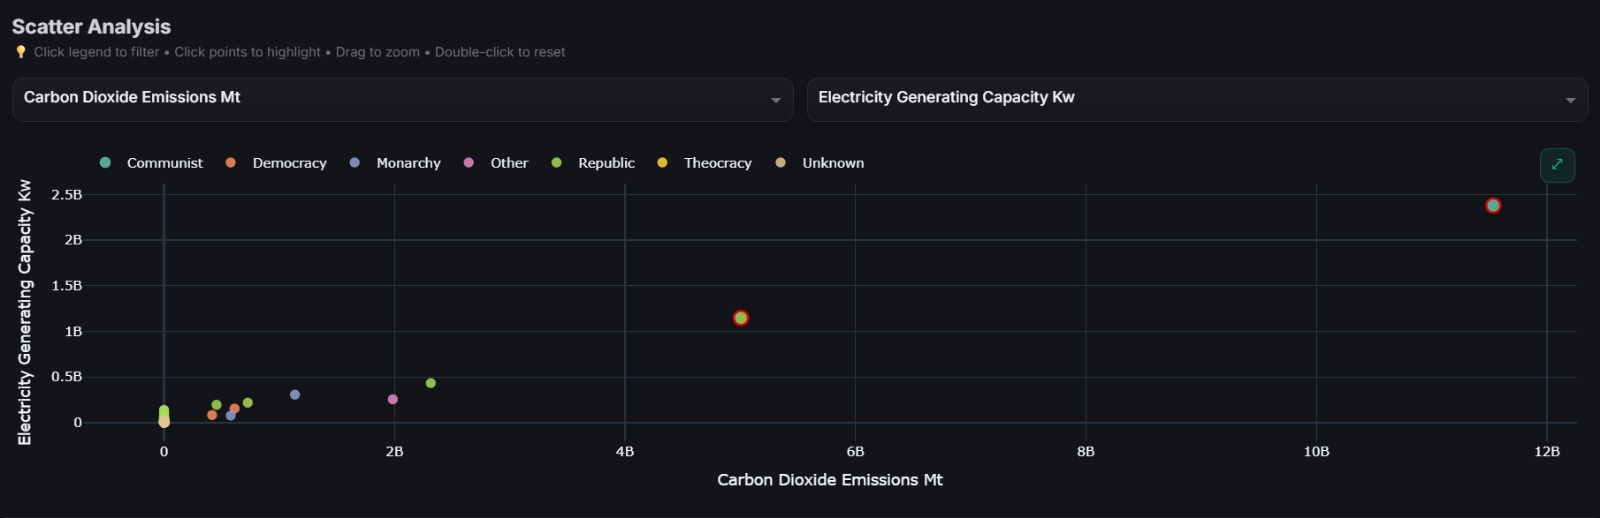
\includegraphics[scale=0.5]{img15.jpeg}
    \caption{Correlation between GDP per Capita and National Electricity Access.}
    \label{fig:global_emissions}
\end{figure}


\textbf{Task 2: Correlate Economic Wealth and Energy Access}
\begin{itemize}
    \item \textbf{Description}: Investigating if wealth alone is a sufficient driver for infrastructure (see Fig.~\ref{fig:wealth_access}).
    \item \textbf{Questions}: Does economic wealth guarantee energy access? Is there a strong correlation between $GDP$ per capita and electricity access?
    \item \textbf{Insight}: Moderate correlation (0.46). Higher GDP helps, but policy and geography are equally critical.
\end{itemize}

% [H] tells LaTeX: "Put this EXACTLY HERE, do not let it float"
\begin{figure}[H]
    \centering
    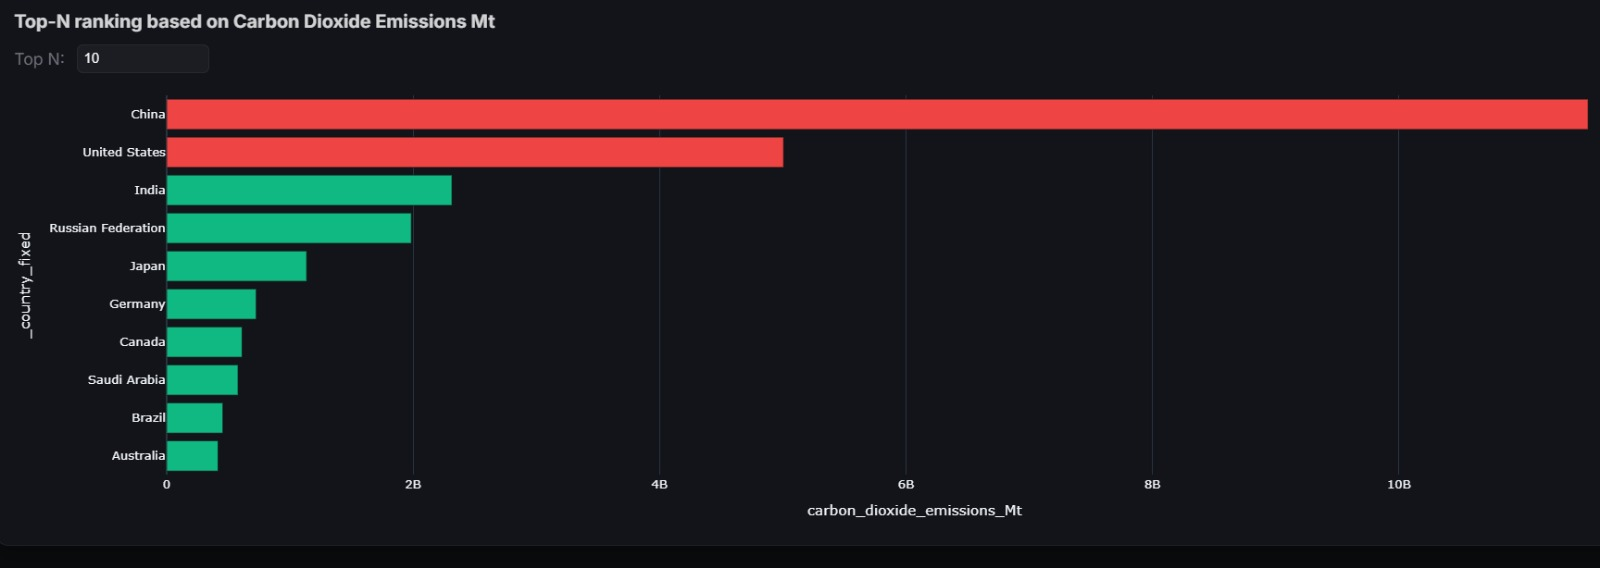
\includegraphics[height=100pt, width=1\linewidth]{fig3.jpeg}
    \caption{Global $CO_{2}$ Emissions vs. Industrial Capacity by Nation.}
    \label{fig:wealth_access}
\end{figure}

\textbf{Task 3: Analyze Carbon Intensity and Economic Efficiency}
\begin{itemize}
    \item \textbf{Description}: Evaluating efficiency by calculating $CO_{2}$ emissions relative to GDP (see Fig.~\ref{fig:carbon_intensity}).
    \item \textbf{Questions}: Which economies are the most "Carbon Intensive"? Who emits the most relative to economic output?
    \item \textbf{Insight}: China and Russia lead major economies. Small island nations show high ratios due to fossil fuel import reliance.
\end{itemize}

% [H] ensures the figure stays directly under the Task 3 bullet points
\begin{figure}[H]
    \centering
    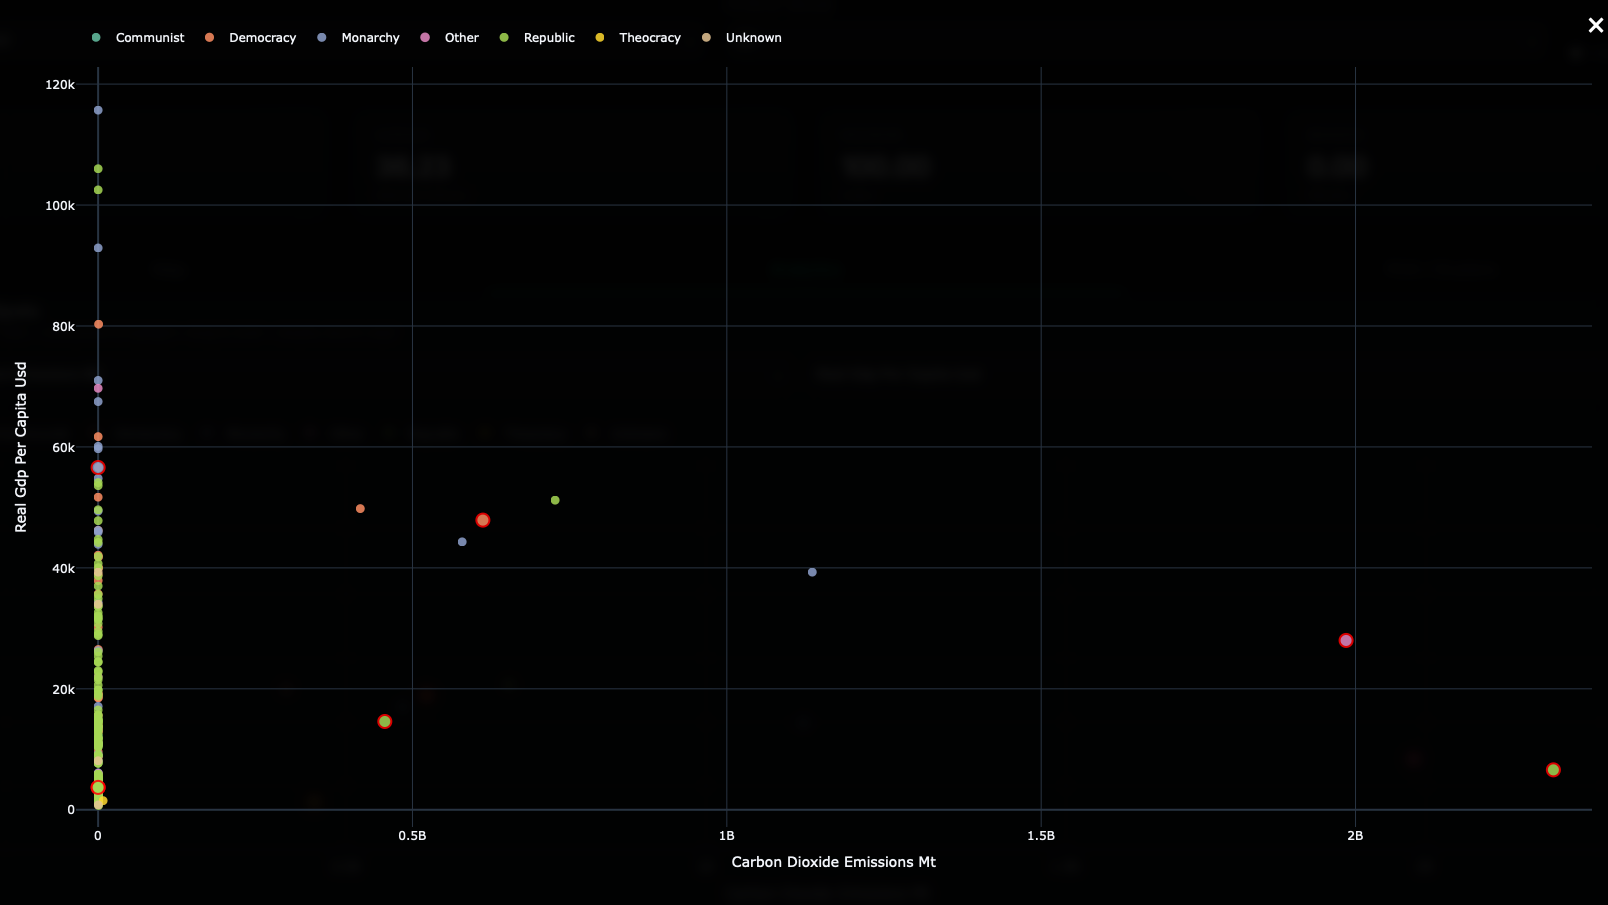
\includegraphics[width=1.0\linewidth]{fig5.png}
    \caption{Real GDP vs Carbon Dioxide Emission Mt.}
    \label{fig:carbon_intensity}
\end{figure}

\begin{figure*}[h] % The * makes it span both columns (large image)
    \centering
    % width=0.9\textwidth makes it wide, height=7cm sets the vertical scale
    % keepaspectratio prevents the image from looking stretched
    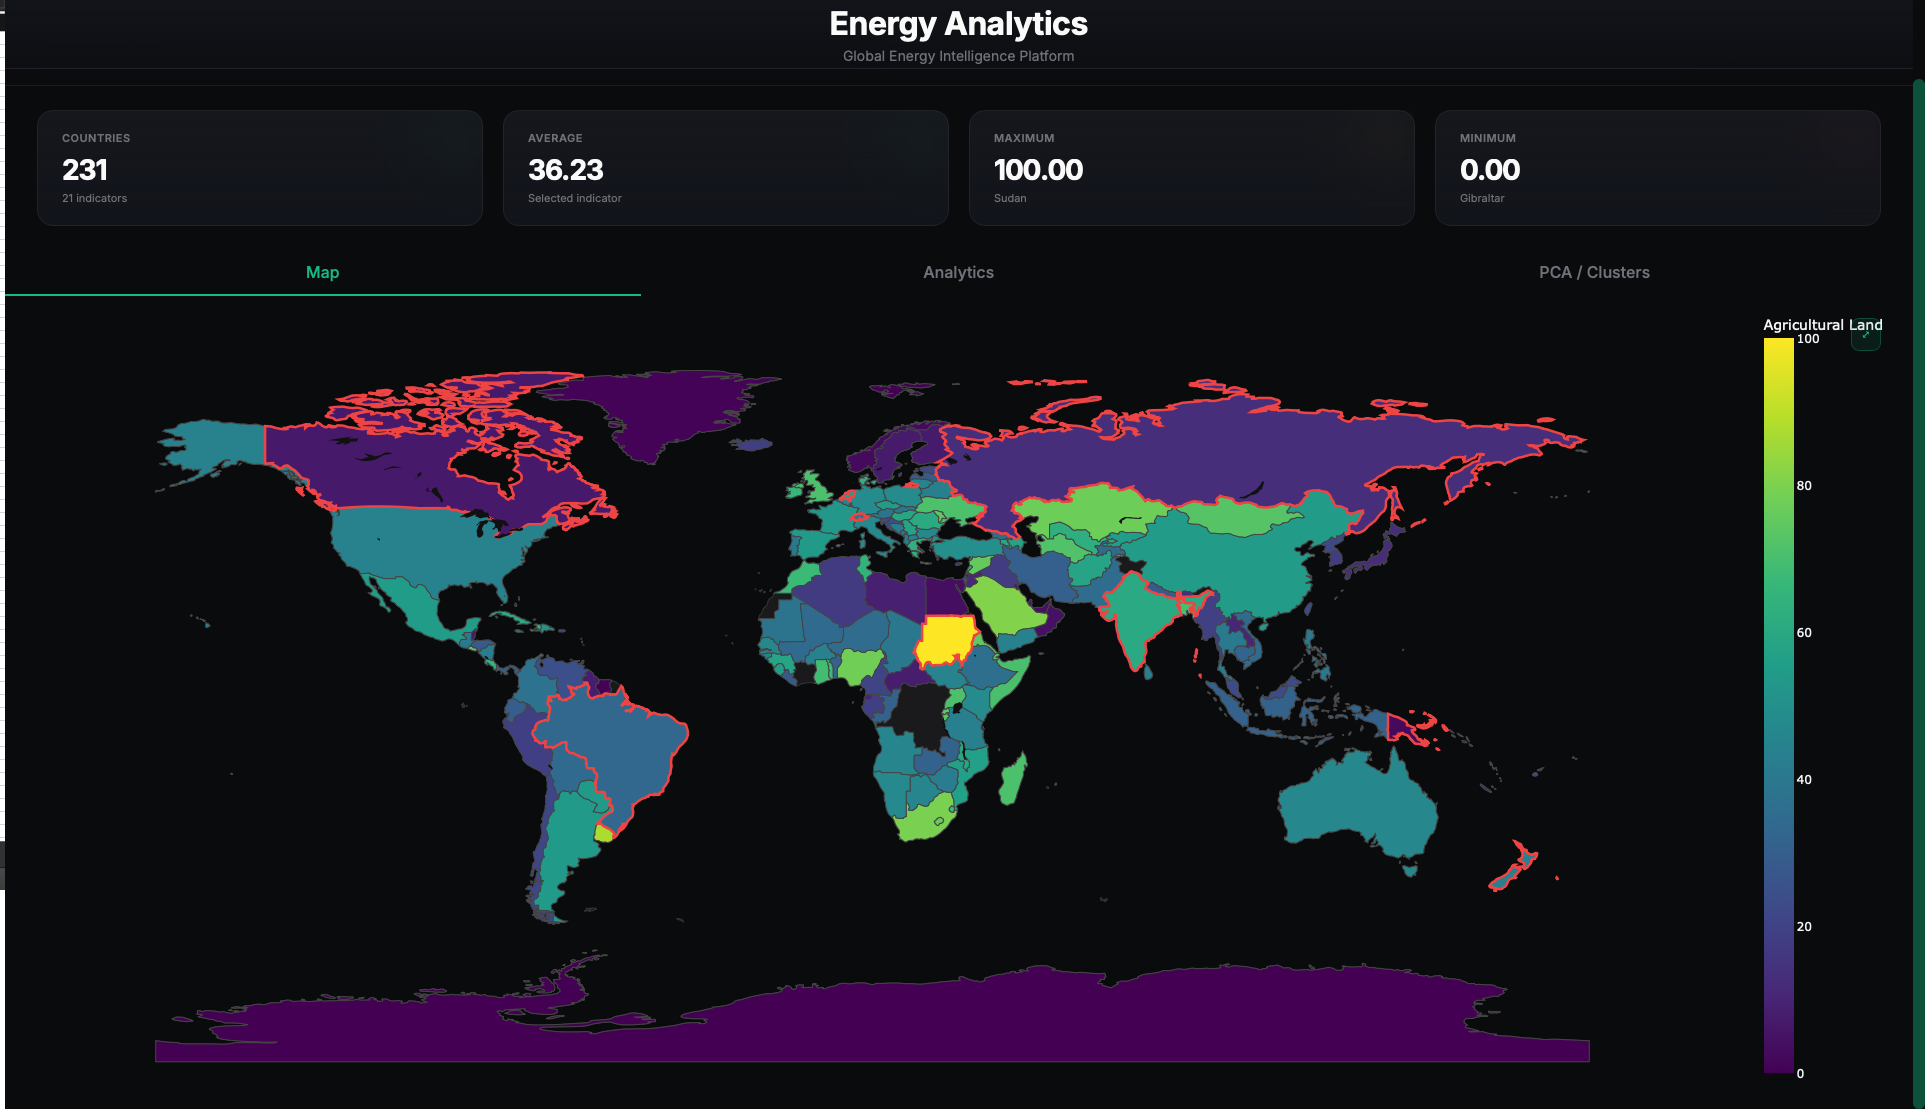
\includegraphics[width=0.9\textwidth, height=10cm, keepaspectratio]{fig9.png} 
        \caption{Agricultural land view through Choropleth Map}
    \label{fig:multivariate_distribution}
\end{figure*}

\begin{table}[H]
\centering
\caption{Task Abstraction: Mapping Domain Tasks to Abstract Actions}
\label{tab:task_abstraction}
\small
\begin{tabular}{|p{1.8cm}|p{1.8cm}|p{1.5cm}|p{2.0cm}|}
\hline
\textbf{Domain Task} & \textbf{Action} & \textbf{Target} & \textbf{Idiom Support} \\
\hline
Discover spatial patterns & Discover & Distribution & Choropleth Map \\
\hline
Generate hypotheses & Discover & Dependency & Scatter Plot \\
\hline
Characterize profiles & Derive & Outliers & PCA + K-Means \\
\hline
Correlate attributes & Identify & Correlation & Scatter Plot, Corr. Matrix \\
\hline
Identify extremes & Identify & Extremes & Bar Chart (Top-N) \\
\hline
Filter by region & Filter & Features & Continent Dropdown \\
\hline
Lookup value & Lookup & Value & Hover Tooltip \\
\hline
Locate country & Locate & Position & Geographic Map \\
\hline
Select \& highlight & Select & Item & Click interaction \\
\hline
Brush range & Filter & Range & Parallel Coordinates \\
\hline
\end{tabular}
\end{table}

\section{Visualization Design}

{\color{blue}
\subsection{Channel Effectiveness Ranking}
Following Munzner's effectiveness rankings, we prioritize channels based on their perceptual accuracy for quantitative data:

\begin{table}[H]
\centering
\caption{Channel Effectiveness Applied to Our Design}
\small
\begin{tabular}{|p{0.8cm}|p{2.5cm}|p{4cm}|}
\hline
\textbf{Rank} & \textbf{Channel} & \textbf{Our Application} \\
\hline
1 & Position & Scatter X/Y, PCA \\
\hline
2 & Length & Bar chart ranking \\
\hline
3 & Area & Bubble size \\
\hline
4 & Color saturation & Choropleth, corr. matrix \\
\hline
5 & Color hue & Continent, clusters \\
\hline
\end{tabular}
\end{table}

\subsection{Marks and Channels per Idiom}

\begin{table}[H]
\centering
\caption{Idiom Justification and Theoretical Mapping}
\label{tab:idiom_justification}
\small
\begin{tabular}{|p{2.2cm}|p{5.5cm}|}
\hline
\textbf{Idiom} & \textbf{Justification (Why we use it)} \\
\hline
Choropleth Map & Encodes data into spatial regions via color to reveal geographic distributions. \\
\hline
Scatter Plot & Best for identifying dependencies/trends using high-precision position channels. \\
\hline
PCA + K-Means & Derives and visualizes hidden clusters within multi-dimensional datasets. \\
\hline
Bar Chart & Uses the length channel for accurate magnitude comparison and ranking. \\
\hline
Corr. Matrix & Provides a high-level summary of all statistical relationships via color saturation. \\
\hline
Parallel Coords & Enables multivariate profiling and range-based filtering via interactive brushing. \\
\hline
\end{tabular}
\end{table}

\begin{table}[H]
\centering
\caption{Visual Encoding Specification}
\scriptsize
\begin{tabular}{|p{1.8cm}|p{1.5cm}|p{2.2cm}|p{1.8cm}|}
\hline
\textbf{Idiom} & \textbf{Mark} & \textbf{Channels} & \textbf{Task} \\
\hline
Choropleth & Area & Color, position & Discover \\
\hline
Scatter Plot & Point & X, Y, color & Correlate \\
\hline
Bar Chart & Line & Length, position & Compare \\
\hline
Parallel Coords & Line & Axis position & Browse \\
\hline
PCA Plot & Point & X, Y, color & Derive \\
\hline
Corr. Matrix & Cell & Color saturation & Identify \\
\hline
\end{tabular}
\end{table}

\subsection{Alternatives Considered}
During design, we evaluated and rejected several alternative encodings:

\textbf{Heatmap Matrix (Countries $\times$ Indicators):} Discarded because with 200+ countries, the matrix becomes visually cluttered and individual cells become too small to distinguish. Scatter plots and parallel coordinates handle high dimensionality more effectively.

\textbf{Radar Charts for Country Profiles:} Rejected because radar charts make it difficult to compare values accurately across items, as the circular layout distorts perception of magnitude. Bar charts provide more accurate comparison.

\textbf{Treemap for Hierarchical Data:} Not suitable because our data lacks a natural hierarchy. Countries are independent items, not nested categories.

\textbf{3D Scatter Plot:} Avoided due to occlusion problems and difficulty in perceiving depth accurately on 2D screens. We use PCA to reduce dimensionality to 2D instead.

\subsection{Perceptual Principles}
Our design applies Gestalt principles to improve comprehension:
\begin{itemize}
    \item \textbf{Proximity:} Related controls are grouped together (e.g., axis selectors near their chart)
    \item \textbf{Similarity:} Consistent colors across views represent the same data (e.g., continent colors)
    \item \textbf{Connection:} Lines in parallel coordinates connect related attribute values for the same country
\end{itemize}

For color scales, we chose Blues (sequential) for the choropleth because it provides good luminance contrast for ordered quantitative data. The correlation matrix uses RdBu (diverging) to distinguish positive correlations (blue) from negative correlations (red), with white at zero. Continent colors use categorical hues with maximum perceptual distance.
}

\subsection{Visual Channel Selection}
Our visual encodings follow Munzner's effectiveness rankings for quantitative data. Position is the most effective channel and is used in scatter plots for X and Y axes, in the PCA embedding, and in the choropleth map for spatial location. Length is used in bar charts for ranking comparison. Color saturation and hue are used in the choropleth with a Blues scale for sequential data, in the correlation matrix with a diverging RdBu scale, and for continent-based coloring across all scatter-based views.

\subsection{Interaction Design}
Linked views support Shneiderman's Visual Information Seeking Mantra of overview first, zoom and filter, then details-on-demand. The choropleth map provides an overview showing global energy distribution at a glance. Zoom and filter capabilities are provided through the continent dropdown that filters all views and through parallel coordinates brushing that narrows the displayed range. Details-on-demand are available through hover tooltips that reveal exact values and through the comparison table that provides detailed country profiles. View linking is achieved by clicking a country on the map, which highlights it in scatter plots, PCA, and parallel coordinates bidirectionally.

{
\color{blue}
\section{Use Case: Energy Analyst Exploration}

This section demonstrates how an energy analyst uses our tool to explore global energy data and discover insights through interaction.

\subsection{Scenario}

An energy analyst at a policy research institute wants to understand the relationship between energy production, carbon emissions, and electricity access. The goal is to find countries that could serve as models for sustainable energy development.

\subsection{Exploration Process}

\textbf{Step 1: Geographic Overview.} The analyst starts with the choropleth map showing Natural Gas distribution (see Fig.~\ref{fig:usecase_map}). The dashboard displays summary statistics: 129 countries, average of 33.5 trillion cubic meters, maximum of 967 trillion (USA), and minimum of 0 (Belgium). Yellow indicates high values, purple indicates low. Russia, Iran, and the US stand out as major gas producers.

\begin{figure}[H]
    \centering
    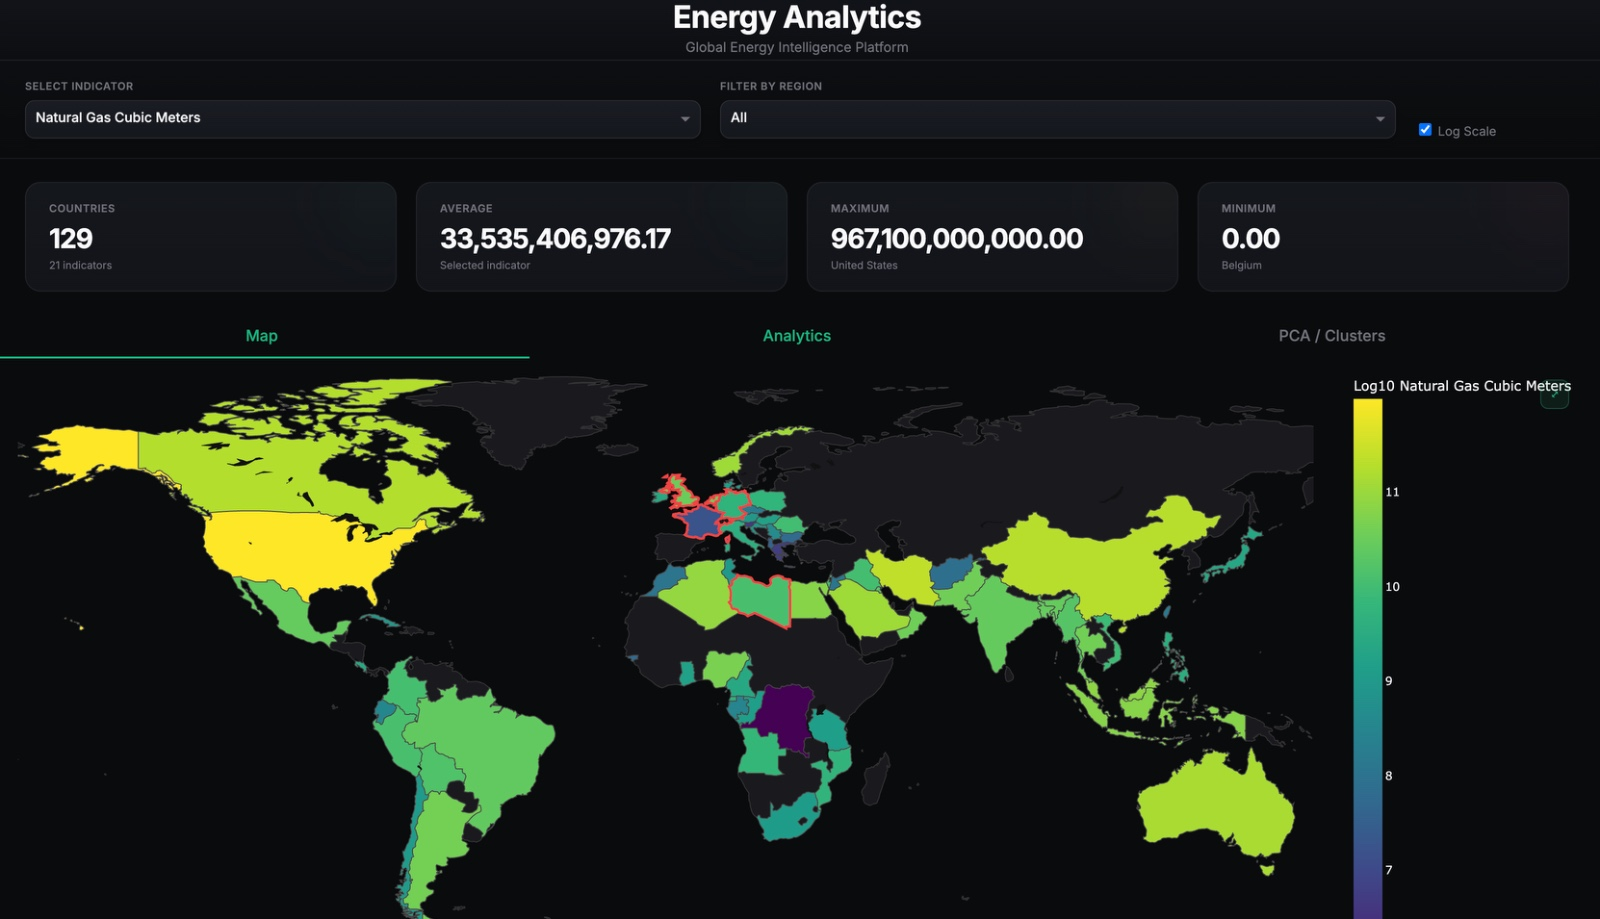
\includegraphics[width=1.0\linewidth]{usecase_step1_worldmap_naturalgas.jpg}
    \caption{Step 1: World map showing Natural Gas distribution with KPI summary cards. The dashboard displays 129 countries, average, maximum (USA), and minimum values.}
    \label{fig:usecase_map}
\end{figure}

\textbf{Step 2: Correlation Discovery.} The analyst switches to the scatter plot to compare Natural Gas reserves against Area Total (see Fig.~\ref{fig:usecase_scatter}). Points are colored by government type---Democracy (orange), Monarchy (gray), Republic (green), etc. Larger countries tend to have more gas reserves, but government type shows interesting clustering patterns. Democracies cluster in the lower-left, while large republics like Russia appear as outliers.

\begin{figure}[H]
    \centering
    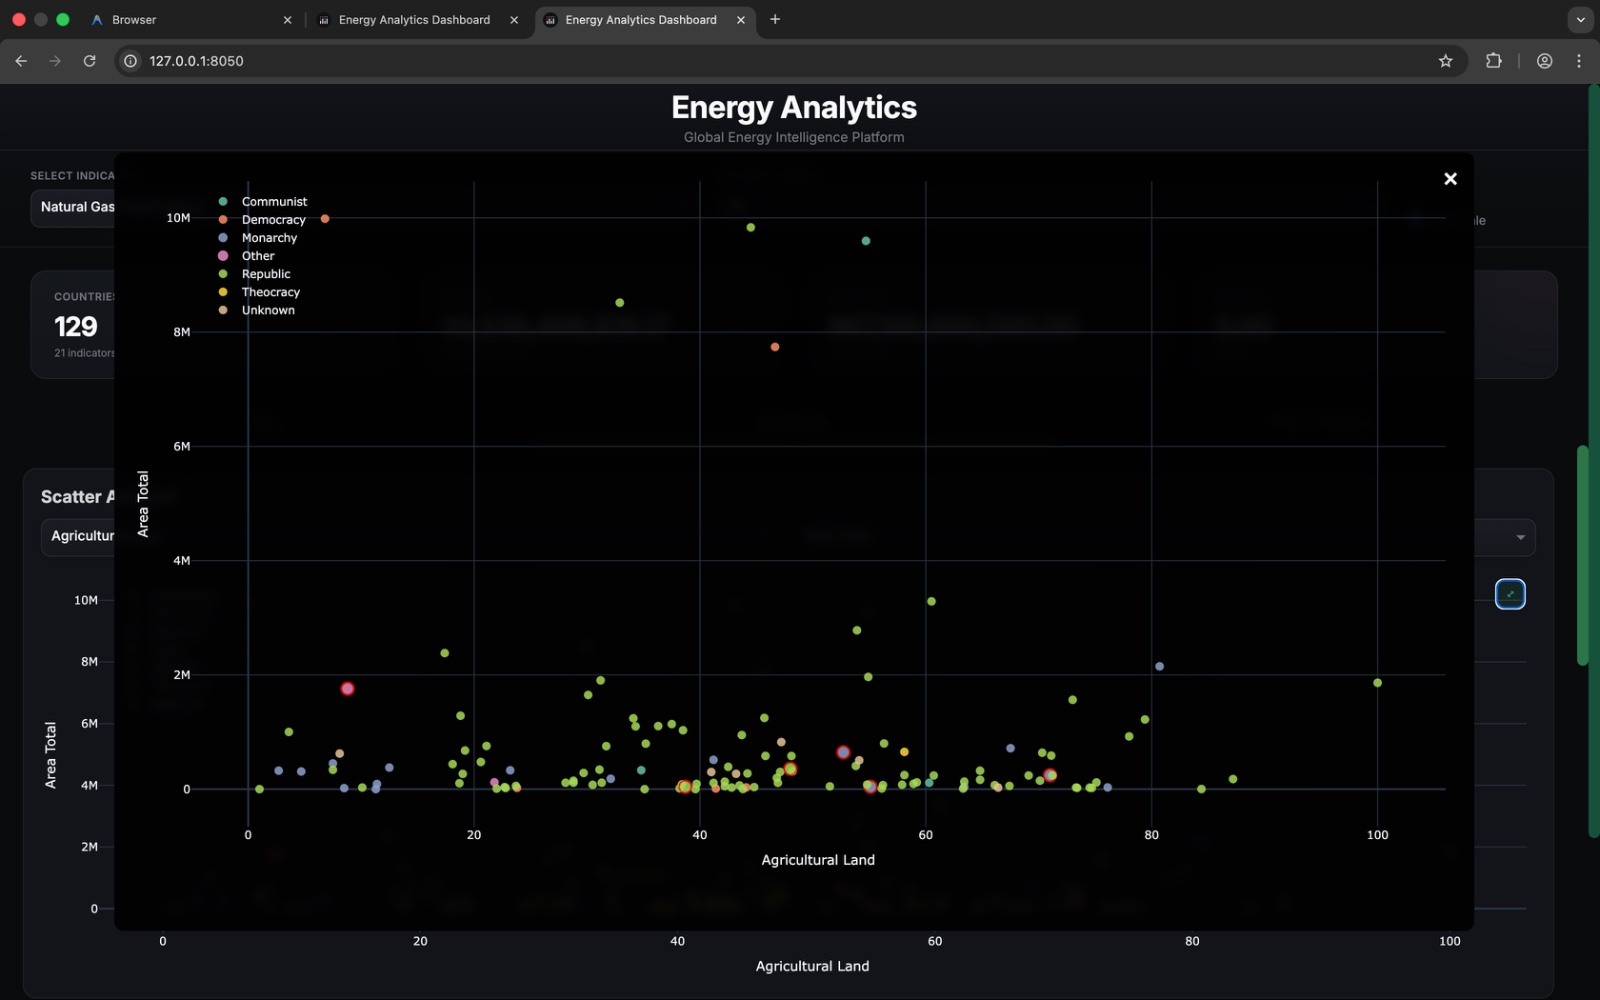
\includegraphics[width=1.0\linewidth]{usecase_step2_scatter_agricultural.jpg}
    \caption{Step 2: Scatter plot of Natural Gas vs Area Total. Points colored by government type (Democracy, Monarchy, Republic, etc.) reveal clustering patterns.}
    \label{fig:usecase_scatter}
\end{figure}

\textbf{Step 3: Multivariate Filtering.} Using parallel coordinates (see Fig.~\ref{fig:usecase_parcoords}), the analyst brushes on ``Real GDP Per Capita'' to select high-income countries. The linked table below shows the brushed countries (Austria, Belgium, etc.) with their attributes. This reveals that high-GDP countries have varying carbon emissions---some achieve prosperity with lower emissions than others.

\begin{figure}[H]
    \centering
    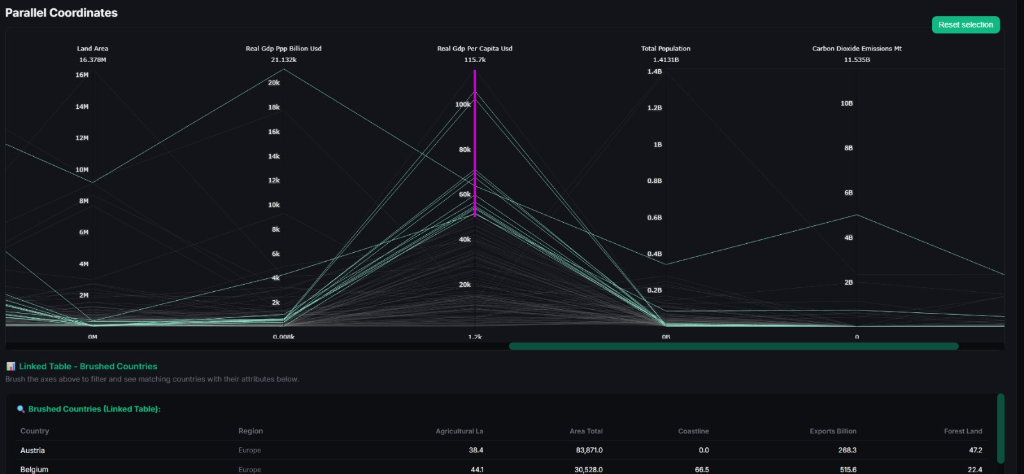
\includegraphics[width=1.0\linewidth]{usecase_step3_parallel_coords.png}
    \caption{Step 3: Parallel coordinates with brushing. Selecting high GDP per capita (pink highlight) filters to wealthy countries shown in linked table.}
    \label{fig:usecase_parcoords}
\end{figure}

\textbf{Step 4: Attribute Correlation.} Finally, the analyst uses the full correlation matrix (see Fig.~\ref{fig:usecase_heatmap}) to explore all pairwise relationships. Strong positive correlations (blue) appear between electricity capacity and coal consumption (0.99), exports and imports (0.93), and petroleum metrics. Negative correlations (red) are rare, indicating most energy indicators move together. This reveals that energy infrastructure is highly interconnected.

\begin{figure}[H]
    \centering
    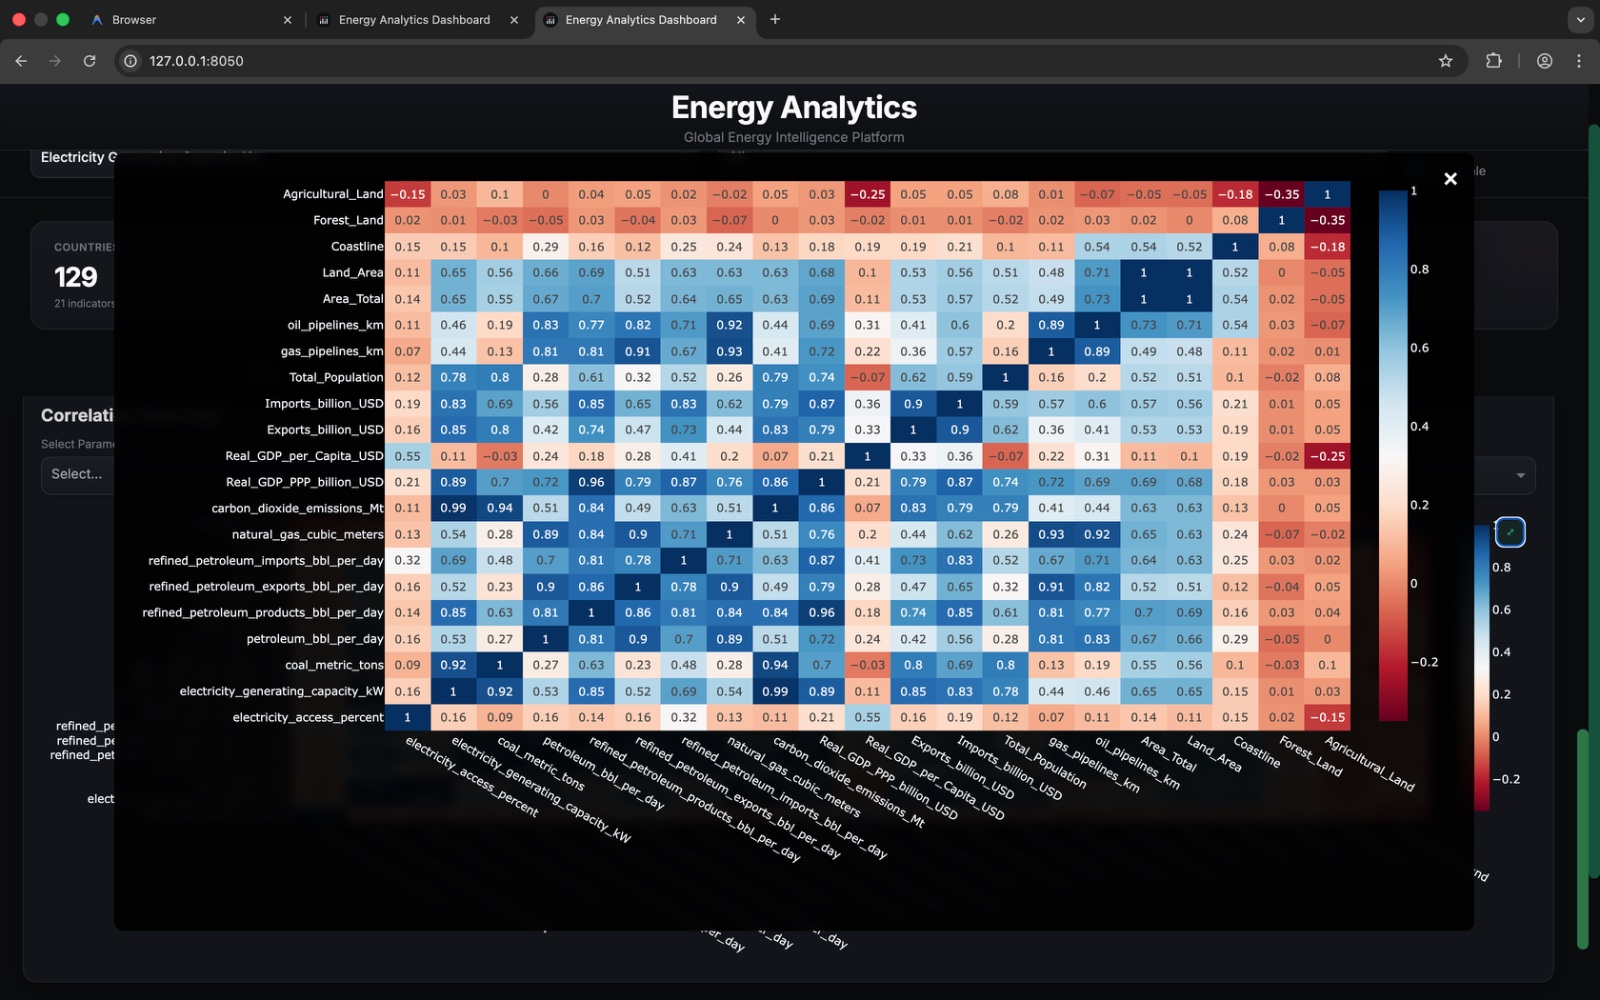
\includegraphics[width=1.0\linewidth]{usecase_step4_correlation_full.jpg}
    \caption{Step 4: Full correlation matrix showing relationships between all attributes. Strong positive correlations appear in blue, negative in red.}
    \label{fig:usecase_heatmap}
\end{figure}

\subsection{Key Findings}

Through this interactive exploration, the analyst discovered:
\begin{enumerate}
    \item \textbf{Decoupling is possible:} Some countries achieve high electricity access with low carbon emissions, suggesting that energy development need not be carbon-intensive.
    \item \textbf{Regional patterns exist:} Geographic clustering of energy access gaps aligns with development status but not always with resource availability.
    \item \textbf{Infrastructure scales with coal:} The 0.92 correlation between coal and electricity capacity shows most countries built infrastructure on fossil fuels.
\end{enumerate}

This exploration demonstrates how linked views and interaction enable hypothesis generation and pattern discovery---tasks that would be difficult with static tables.
}

{
\color{blue}
\section{Implementation}

\subsection{Technology Stack}
The tool is built entirely in Python using:
\begin{itemize}
    \item \textbf{Dash:} Web-based UI framework for building analytical applications
    \item \textbf{Plotly:} Interactive visualization library for charts and maps
    \item \textbf{Pandas:} Data manipulation and cleaning with regex preprocessing
    \item \textbf{Scikit-learn:} PCA dimensionality reduction and K-Means clustering
    \item \textbf{pycountry / pycountry-convert:} ISO code and continent inference
    \item \textbf{gapminder:} Country name standardization and matching
\end{itemize}

\subsection{View Coordination}
Multi-view coordination is achieved through Dash callbacks that link component states. When a user clicks a country on the map, the \texttt{clickData} event triggers updates to scatter plots, PCA, and parallel coordinates. A shared \texttt{dcc.Store} component maintains the selected countries, enabling bidirectional linking between all views.

\subsection{Technical Challenges}
We encountered several challenges during development:
\begin{itemize}
    \item \textbf{Inconsistent country names:} CIA database uses different naming conventions than ISO standards. We built a custom matching table to resolve discrepancies (e.g., ``Czechia'' $\rightarrow$ ``Czech Republic'').
    \item \textbf{Missing data:} Approximately 15\% of values are missing. We exclude these from individual visualizations rather than imputing to preserve accuracy.
    \item \textbf{Map stability:} Maintaining consistent map display during brushing interactions required careful state management.
    \item \textbf{Dark theme UI:} Designing readable visualizations on dark backgrounds with proper contrast and animated transitions.
\end{itemize}

\section{Conclusion and Future Work}

\subsection{Summary of Results}

We built an interactive visualization tool that lets energy analysts explore the CIA World Factbook dataset across 200+ countries. The tool supports tasks from high-level pattern discovery to detailed value lookup through linked views: choropleth maps, scatter plots, parallel coordinates, PCA clustering, and bar charts.

\subsection{Benefits and Limitations}

\textbf{Benefits:}
\begin{itemize}
    \item Linked views let analysts move from overview to detail quickly
    \item Multiple chart types support different tasks (comparison, correlation, clustering)
    \item Interactive filtering through selection and brushing
    \item Dark theme with smooth animations
\end{itemize}

\textbf{Limitations:}
\begin{itemize}
    \item Single point in time---no temporal trends
    \item 15\% missing values reduce coverage for some countries
    \item No derived metrics (e.g., emissions per capita)
\end{itemize}

\subsection{Reflection on Design Choices}

The choropleth map worked well for showing spatial patterns like electricity access gaps. However, for attributes without geographic patterns (e.g., natural gas production), a sorted bar chart would be better.

The parallel coordinates view is powerful for multivariate filtering but suffers from axis overlap with many indicators. Allowing users to reorder or hide axes would help. PCA clustering revealed country groupings but lacks interpretability---adding loading vectors would show which attributes drive cluster separation.

\subsection{Future Work}

Several enhancements would improve the tool:
\begin{itemize}
    \item \textbf{Temporal slider:} Add historical data to track how country profiles evolve
    \item \textbf{Derived metrics:} Compute per-capita and efficiency ratios
    \item \textbf{Axis reordering:} Let users drag parallel coordinates axes
    \item \textbf{Export:} Allow analysts to export filtered data subsets
    \item \textbf{Guided tours:} Provide preset exploration paths for new users
\end{itemize}
}

{\color{blue}
\begin{thebibliography}{00}
\bibitem{munzner2014} T. Munzner, ``Visualization Analysis and Design,'' A K Peters/CRC Press, 2014.
\bibitem{shneiderman1996} B. Shneiderman, ``The eyes have it: a task by data type taxonomy for information visualizations,'' in Proceedings 1996 IEEE Symposium on Visual Languages, pp. 336-343, 1996.
\bibitem{plotly} Plotly Technologies Inc., ``Plotly Python Graphing Library,'' \url{https://plotly.com/python/}, 2024.
\bibitem{dash} Plotly Technologies Inc., ``Dash: A Python Framework for Building Analytical Web Applications,'' \url{https://dash.plotly.com/}, 2024.
\bibitem{cia} Central Intelligence Agency, ``The World Factbook,'' \url{https://www.cia.gov/the-world-factbook/}, 2024.
\bibitem{sklearn} F. Pedregosa et al., ``Scikit-learn: Machine Learning in Python,'' Journal of Machine Learning Research, vol. 12, pp. 2825-2830, 2011. (Used for PCA and K-Means clustering)
\bibitem{pandas} W. McKinney, ``Data Structures for Statistical Computing in Python,'' in Proceedings of the 9th Python in Science Conference, pp. 51-56, 2010.
\bibitem{pycountry} ``pycountry: ISO country, subdivision, language, currency and script definitions,'' \url{https://pypi.org/project/pycountry/}, 2024.
\end{thebibliography}
}

\newpage

\section{Appendix}
\begin{figure*}
    \centering
    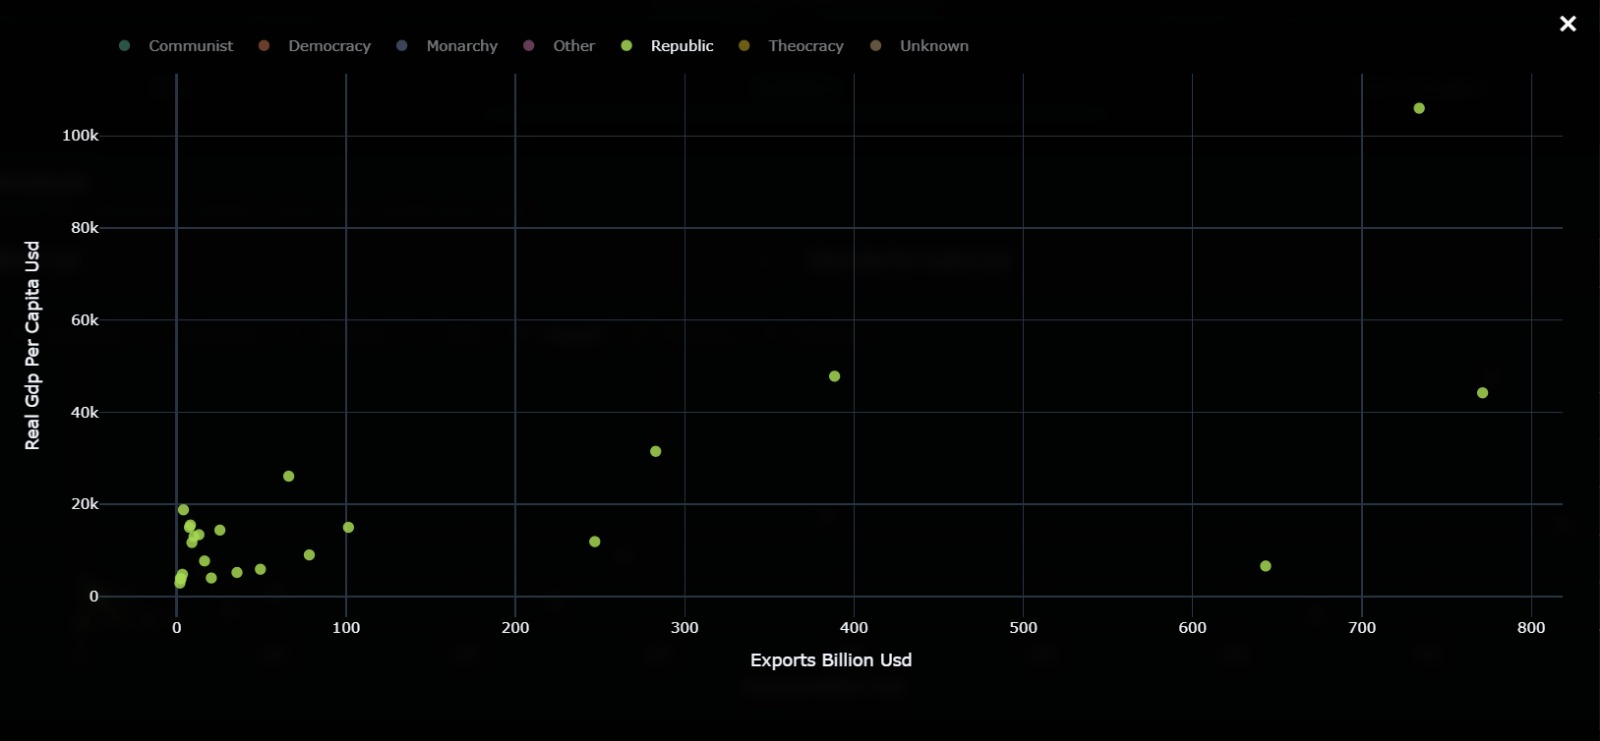
\includegraphics[width=1.0\linewidth]{img16.jpeg}
    \caption{Scatter Analysis for Real GDP vs Exports Billion usd (Government type selection)}
    \label{fig:appendix1}
\end{figure*}

\begin{figure*}
    \centering
    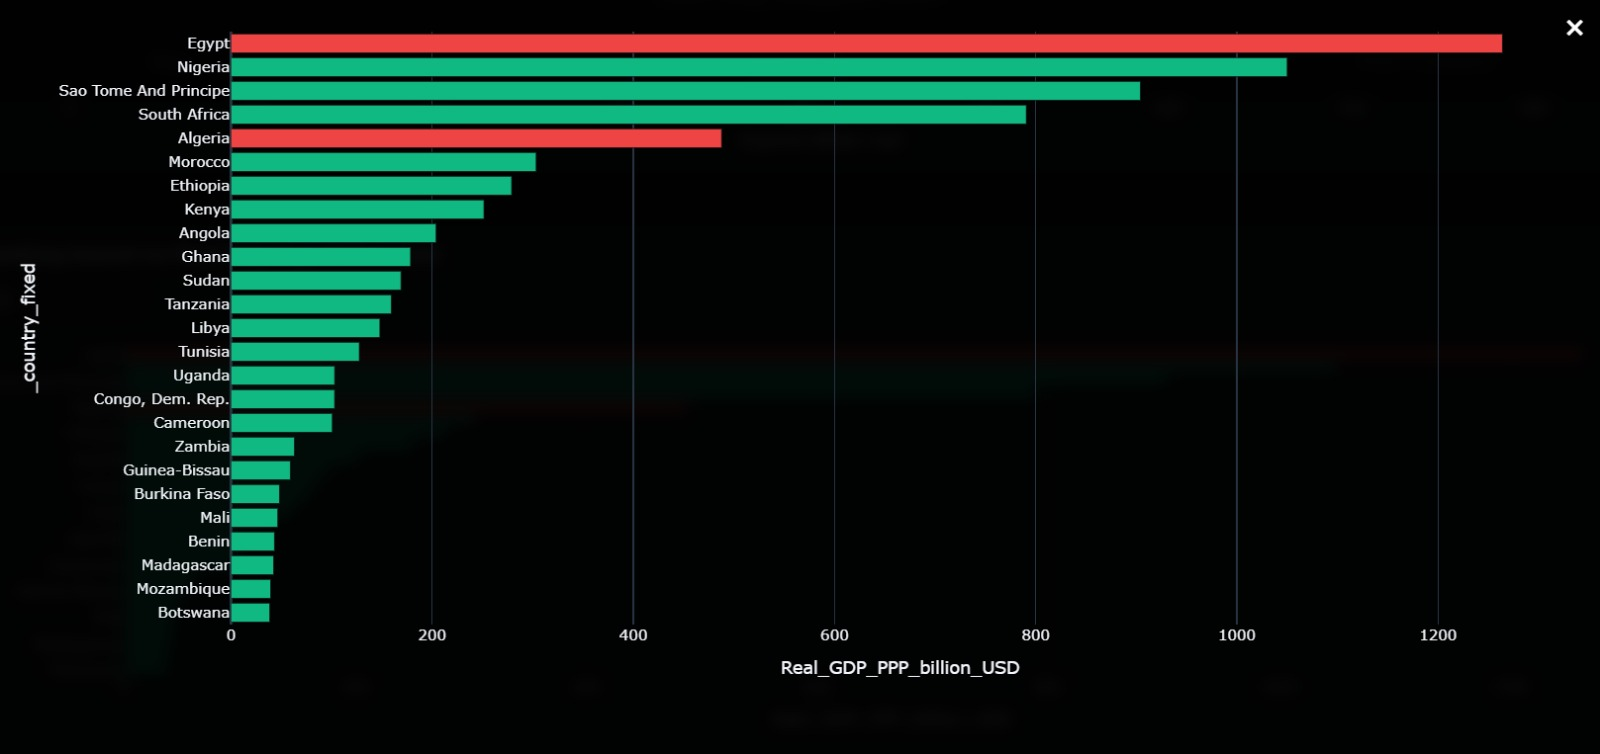
\includegraphics[width=1.0\linewidth]{img 20.jpeg}
    \caption{Top 25 Real GDP for different Countries}
    \label{fig:appendix2}
\end{figure*}

\begin{figure*}
    \centering
    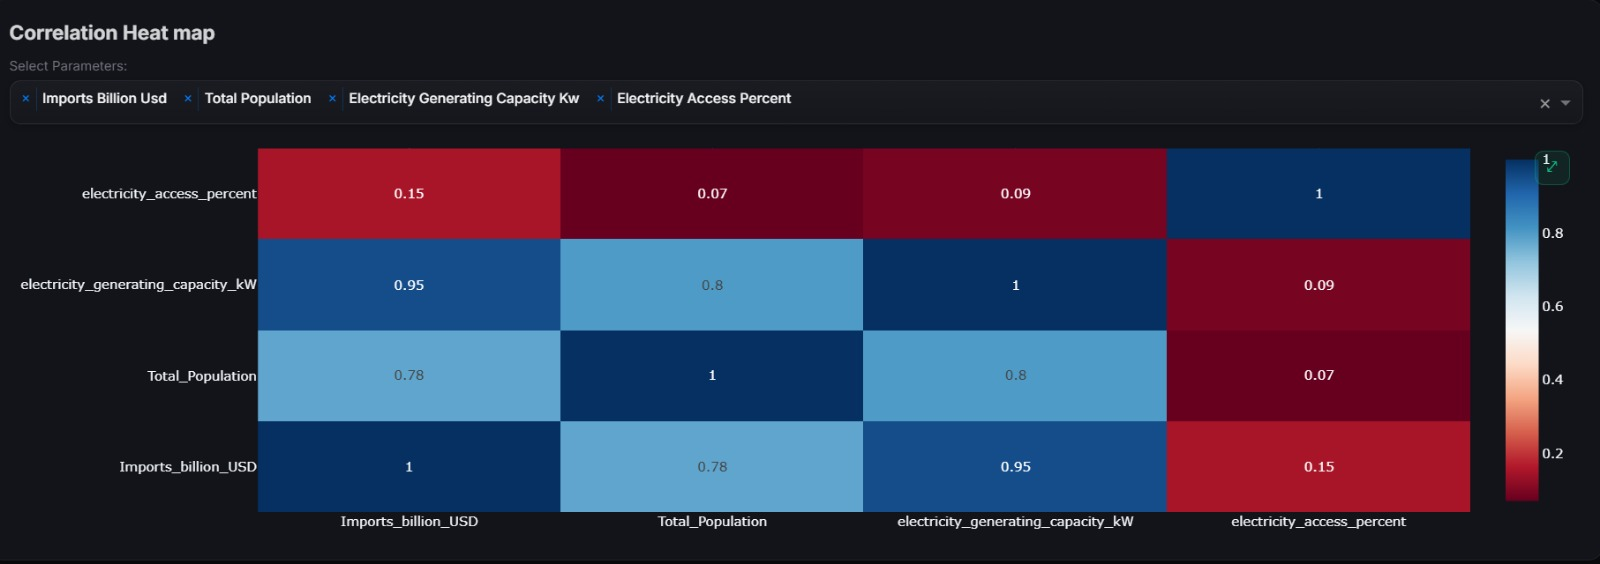
\includegraphics[width=1.0\linewidth]{img18.jpeg}
    \caption{Correlation Heatmap}
    \label{fig:appendix3}
\end{figure*}

\begin{figure*}
    \centering
    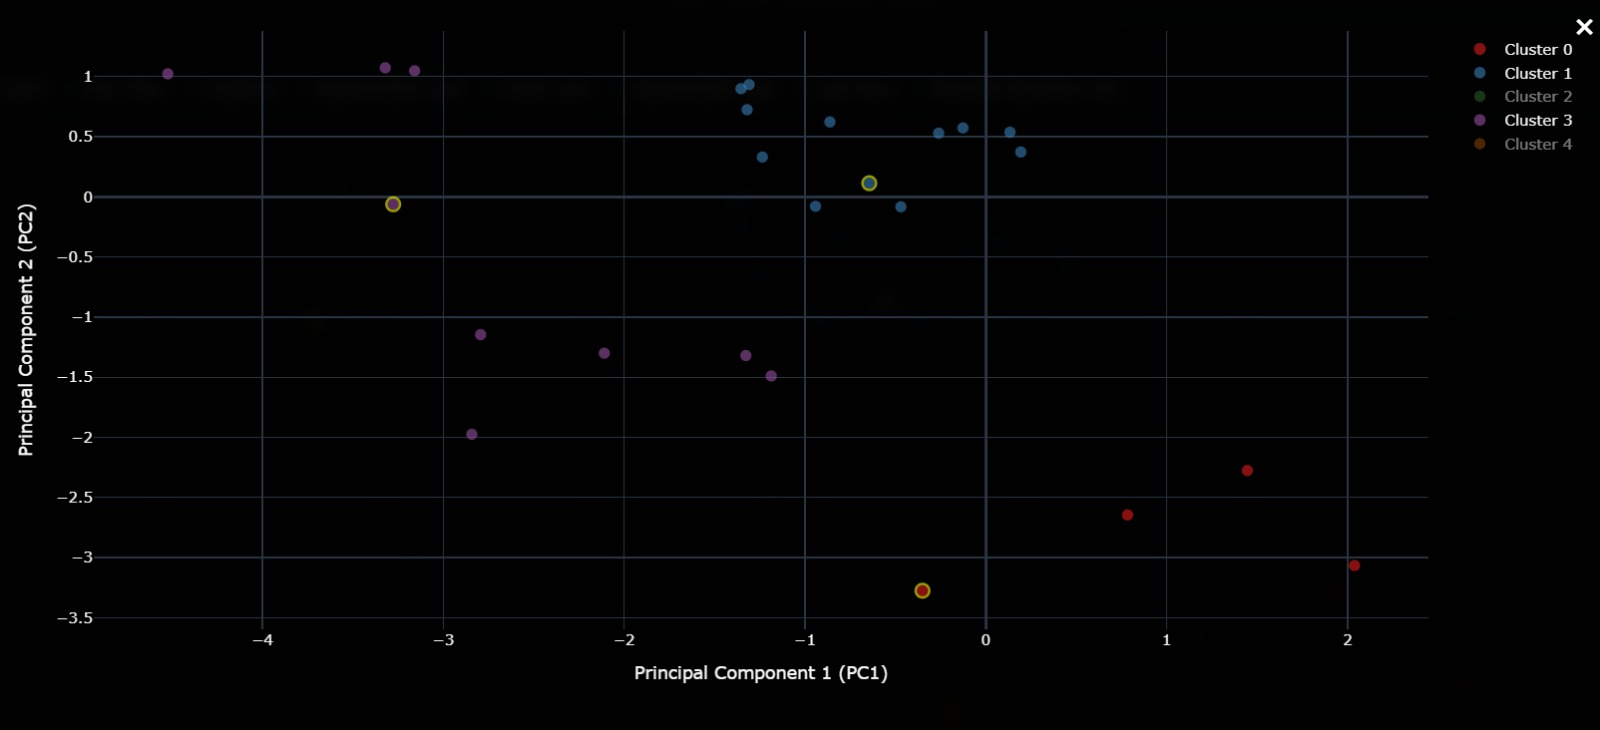
\includegraphics[width=1.0\linewidth]{img19.jpeg}
    \caption{PCA Analysis for Africa (cluster selection)}
    \label{fig:appendix4}
\end{figure*}


\end{document}